\documentclass[aspectratio=169,10pt]{beamer}

\usepackage[T1]{fontenc}
\usepackage{lmodern}
\usepackage{amsmath,amssymb,bm}
\usepackage{graphicx}
\usepackage{booktabs,tabularx,array}
\usepackage{siunitx}
\usepackage{xcolor}

\graphicspath{{figures/}}
\sisetup{detect-all,group-separator={,},group-minimum-digits=4}

\definecolor{hfblue}{RGB}{21,73,125}
\definecolor{hflight}{RGB}{232,241,250}
\definecolor{hforange}{RGB}{230,104,36}
\definecolor{hfgreen}{RGB}{34,126,94}
\setbeamercolor{structure}{fg=hfblue}
\setbeamercolor{frametitle}{fg=white,bg=hfblue}
\setbeamercolor{block title}{fg=white,bg=hfblue}
\setbeamercolor{block body}{fg=black,bg=hflight}
\setbeamercolor{alerted text}{fg=hforange}
\setbeamertemplate{navigation symbols}{}
\setbeamertemplate{itemize item}{\color{hforange}$\blacktriangleright$}
\setbeamertemplate{footline}{%
  \leavevmode\hbox{%
  \begin{beamercolorbox}[wd=.78\paperwidth,ht=2.7ex,dp=1.1ex,leftskip=1em]{author in head/foot}%
    GPU-Accelerated Physics-Based Urban Flood Modelling
  \end{beamercolorbox}%
  \begin{beamercolorbox}[wd=.22\paperwidth,ht=2.7ex,dp=1.1ex,rightskip=1em plus1fil]{date in head/foot}%
    \insertframenumber/15
  \end{beamercolorbox}}
}
\setbeamertemplate{caption}{\raggedright\insertcaption\par}
\setbeamerfont{caption}{size=\tiny}
\setlength{\tabcolsep}{4pt}

\newcommand{\evsource}{\par\vspace{1mm}{\tiny\color{gray}Source: \texttt{HF\_CUPY\_JAX\_COMPLETED\_PROJECT}.}}
\newcommand{\tightitem}{\setlength\itemsep{2pt}\setlength\parskip{0pt}}

\title{GPU-Accelerated Physics-Based\\Urban Flood Modelling}
\subtitle{A production comparison of CuPy/CUDA and JAX/XLA}
\author{Sanjeev Kumawat}
\institute{M.Sc. Student, Indian Institute of Technology Hyderabad\\[2mm]
Under the guidance of Udit Bhatia\\Associate Professor, Indian Institute of Gandhinagar}
\date{August 2026}

\begin{document}

% 1
\begin{frame}[plain]
  \centering
  \vspace{2mm}
  {\usebeamerfont{title}\color{hfblue}\bfseries\inserttitle\par}
  \vspace{2mm}
  {\large\insertsubtitle\par}
  \vspace{7mm}
  {\normalsize\textbf{Sanjeev Kumawat}\par}
  {\small M.Sc. Student, Indian Institute of Technology Hyderabad\par}
  \vspace{5mm}
  {\small Under the guidance of \textbf{Udit Bhatia}\par}
  {\small Associate Professor, Indian Institute of Gandhinagar\par}
  \vspace{6mm}
  
\includegraphics[height=13mm]{iitgn_logo.png}\hspace{8mm}
  
\includegraphics[height=13mm]{iith_logo.png}
  \vfill
  {\small INSPIRE Summer Project \hfill August 2026\par}
\end{frame}

% 2
\begin{frame}{1. Research question and completed contribution}
\begin{block}{Central question}
Can two GPU programming systems execute the same city-scale physics-based flood model and
remain numerically equivalent under predefined scientific criteria?
\end{block}

The completed study implements one production model through \textbf{CuPy/CUDA} and
\textbf{JAX/XLA}. Both paths use the same mesh, terrain, resistance, rainfall, infiltration,
drainage, recharge, boundary forcing, precision and output schedule.

\vspace{3mm}
\begin{columns}[T,onlytextwidth]
\column{0.48\textwidth}
\textbf{Completed evidence}
\begin{itemize}\tightitem
\item Full 24-hour production runs on one GPU
\item Cross-backend parity and repeatability
\item Mass-ledger and software verification
\item Repeated secondary GPU benchmark
\end{itemize}
\column{0.48\textwidth}
\textbf{Scientific interpretation}

The evidence establishes implementation correctness and numerical consistency. It does not
convert model output into observed flood truth; physical accuracy remains a separate
validation question.
\end{columns}
\evsource
\end{frame}

% 3
\begin{frame}{2. Production domain and drainage network}
\begin{columns}[T,onlytextwidth]
\column{0.60\textwidth}
\begin{columns}[T,onlytextwidth]
\column{0.50\textwidth}
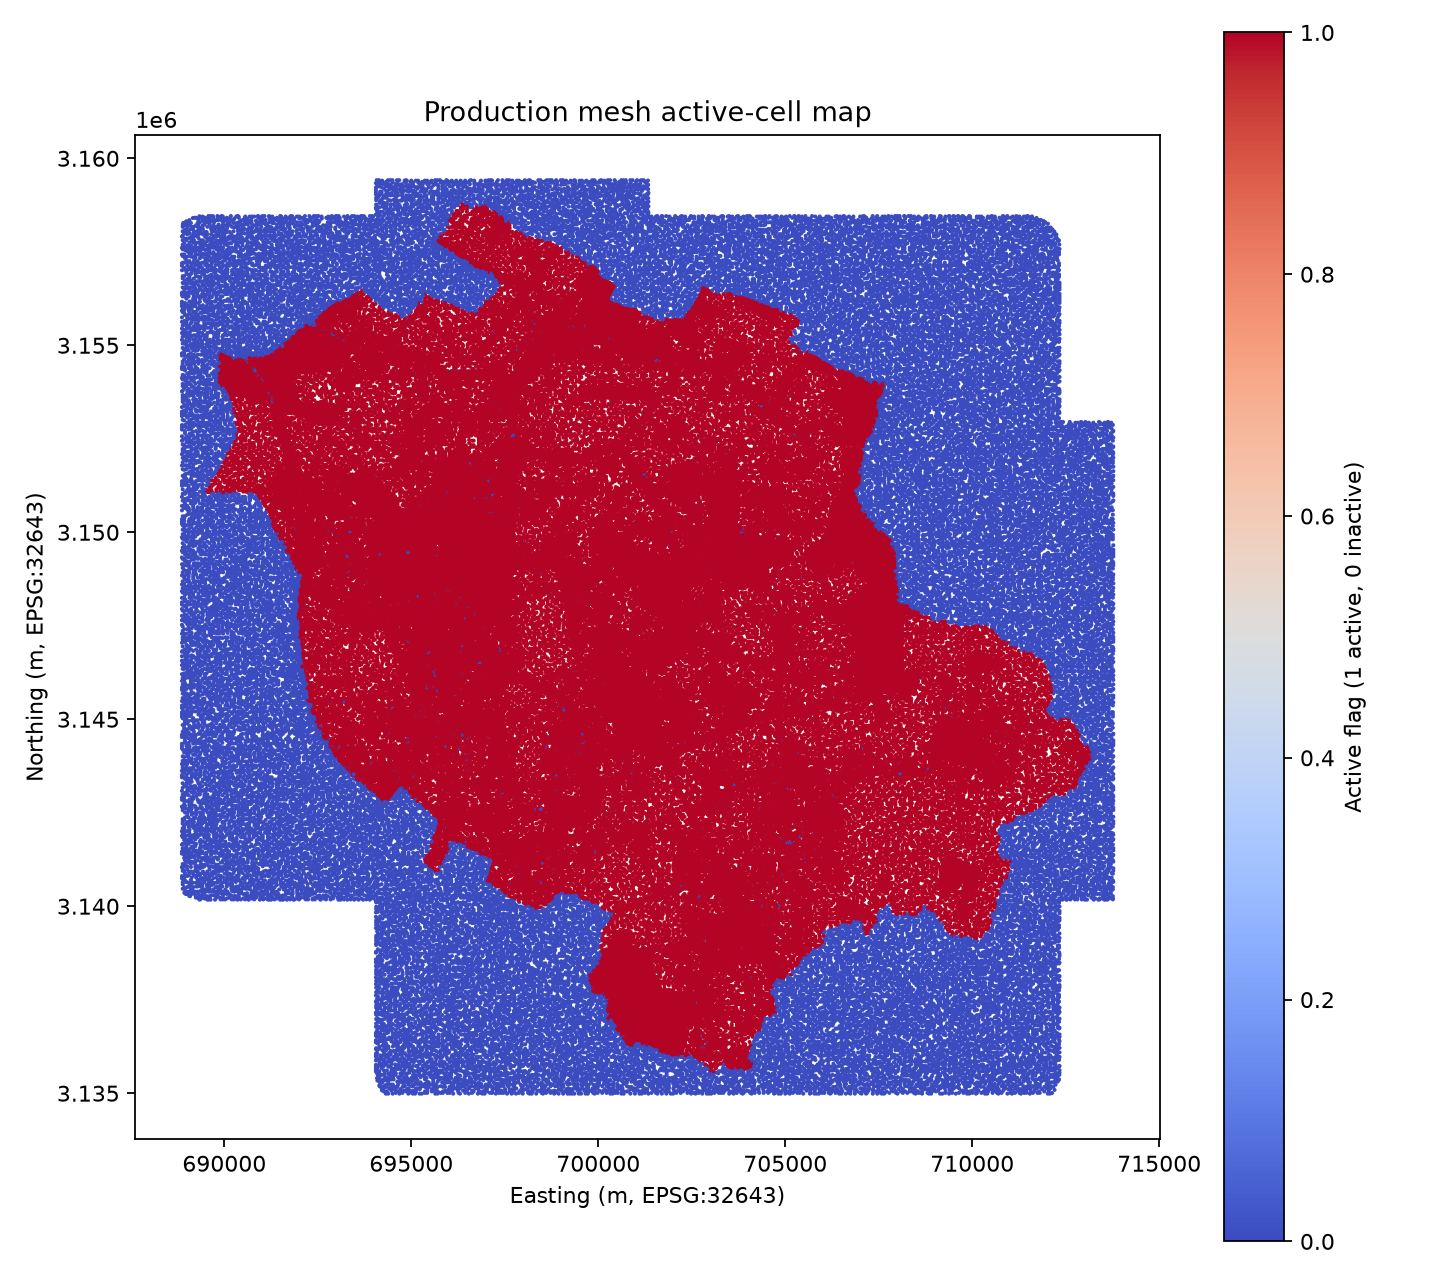
\includegraphics[width=\linewidth]{01_mesh_active_cells.png}
\centering{\tiny Active and inactive surface triangles}
\column{0.50\textwidth}
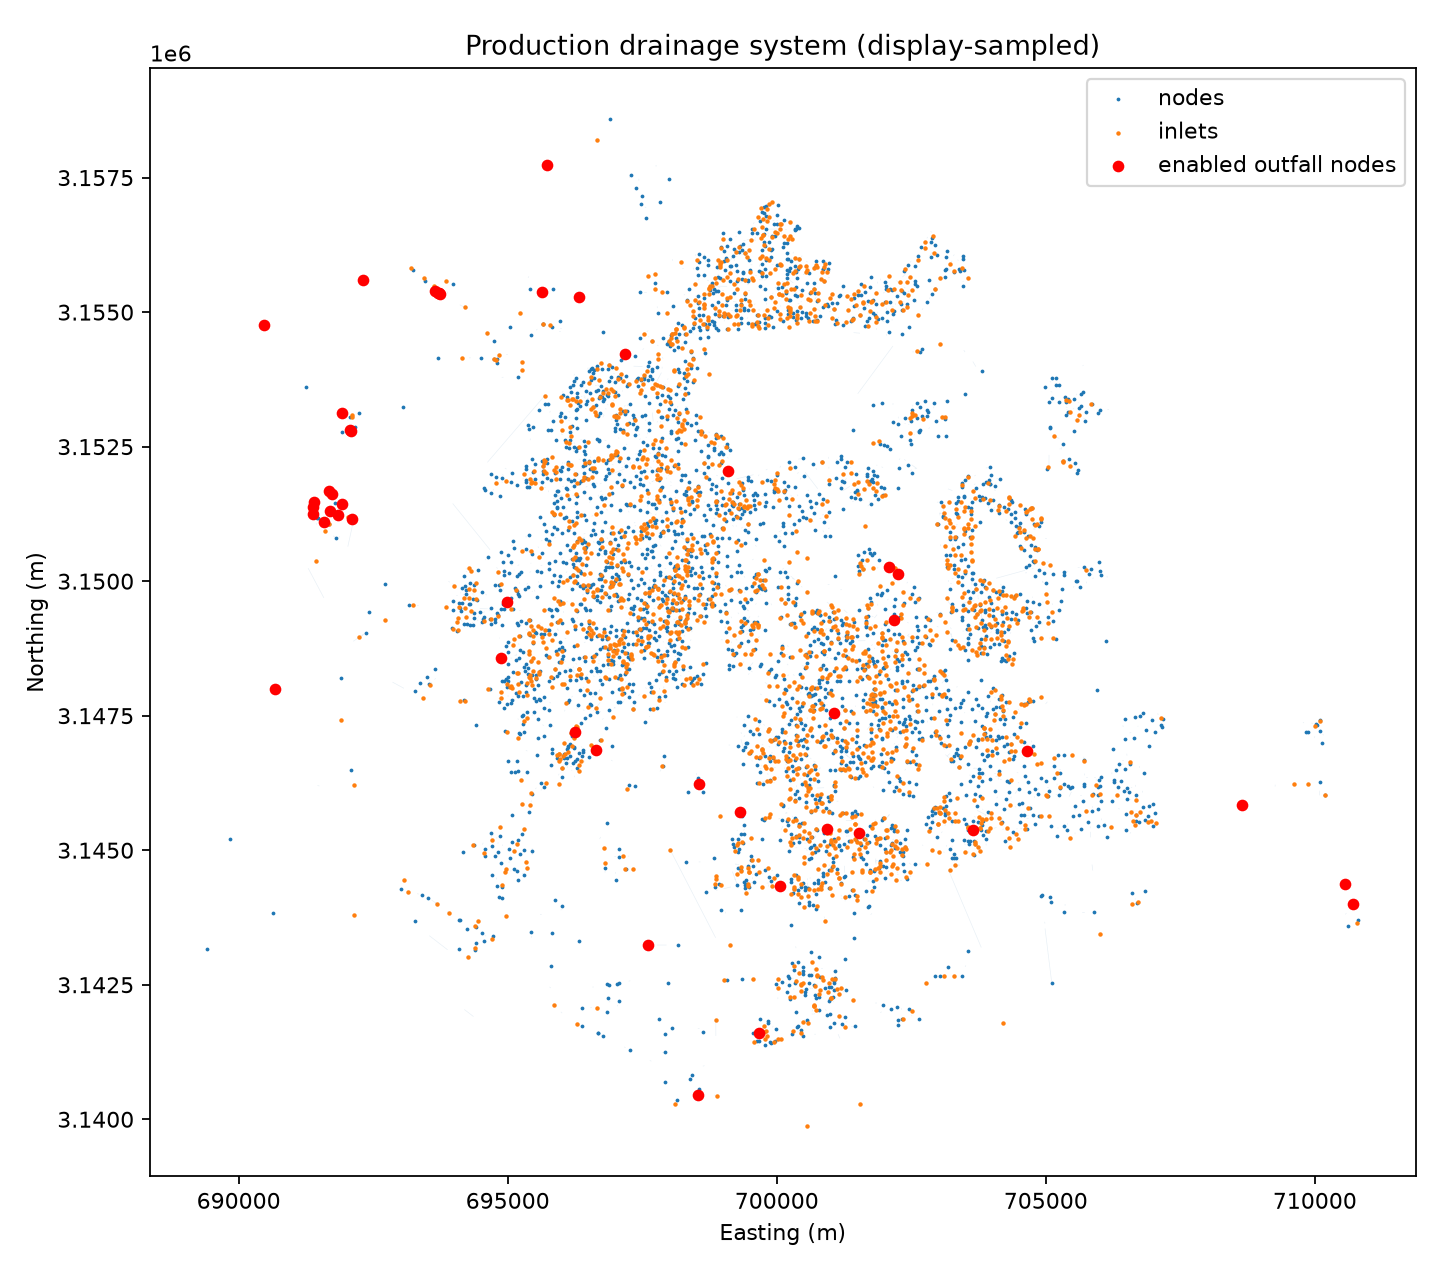
\includegraphics[width=\linewidth]{07_drainage.png}
\centering{\tiny Surface-associated drainage network}
\end{columns}
\column{0.37\textwidth}
\small
\begin{tabular}{@{}lr@{}}
\toprule
Mesh vertices & 499,901\\
Triangles & 981,880\\
Active triangles & 817,573\\
Surface edges & 1,490,015\\
Active area & 297.966 km$^2$\\
Exterior edges & 34,390\\
\midrule
Drainage nodes & 118,768\\
Drainage links & 139,798\\
Mapped inlets & 61,317\\
Enabled outfalls & 46\\
Recharge records & 447\\
\bottomrule
\end{tabular}

\vspace{2mm}
Projected coordinate system: \textbf{EPSG:32643}.
\end{columns}
\evsource
\end{frame}

% 4
\begin{frame}{3. Terrain, resistance and rainfall inputs}
\begin{columns}[T,onlytextwidth]
\column{0.32\textwidth}
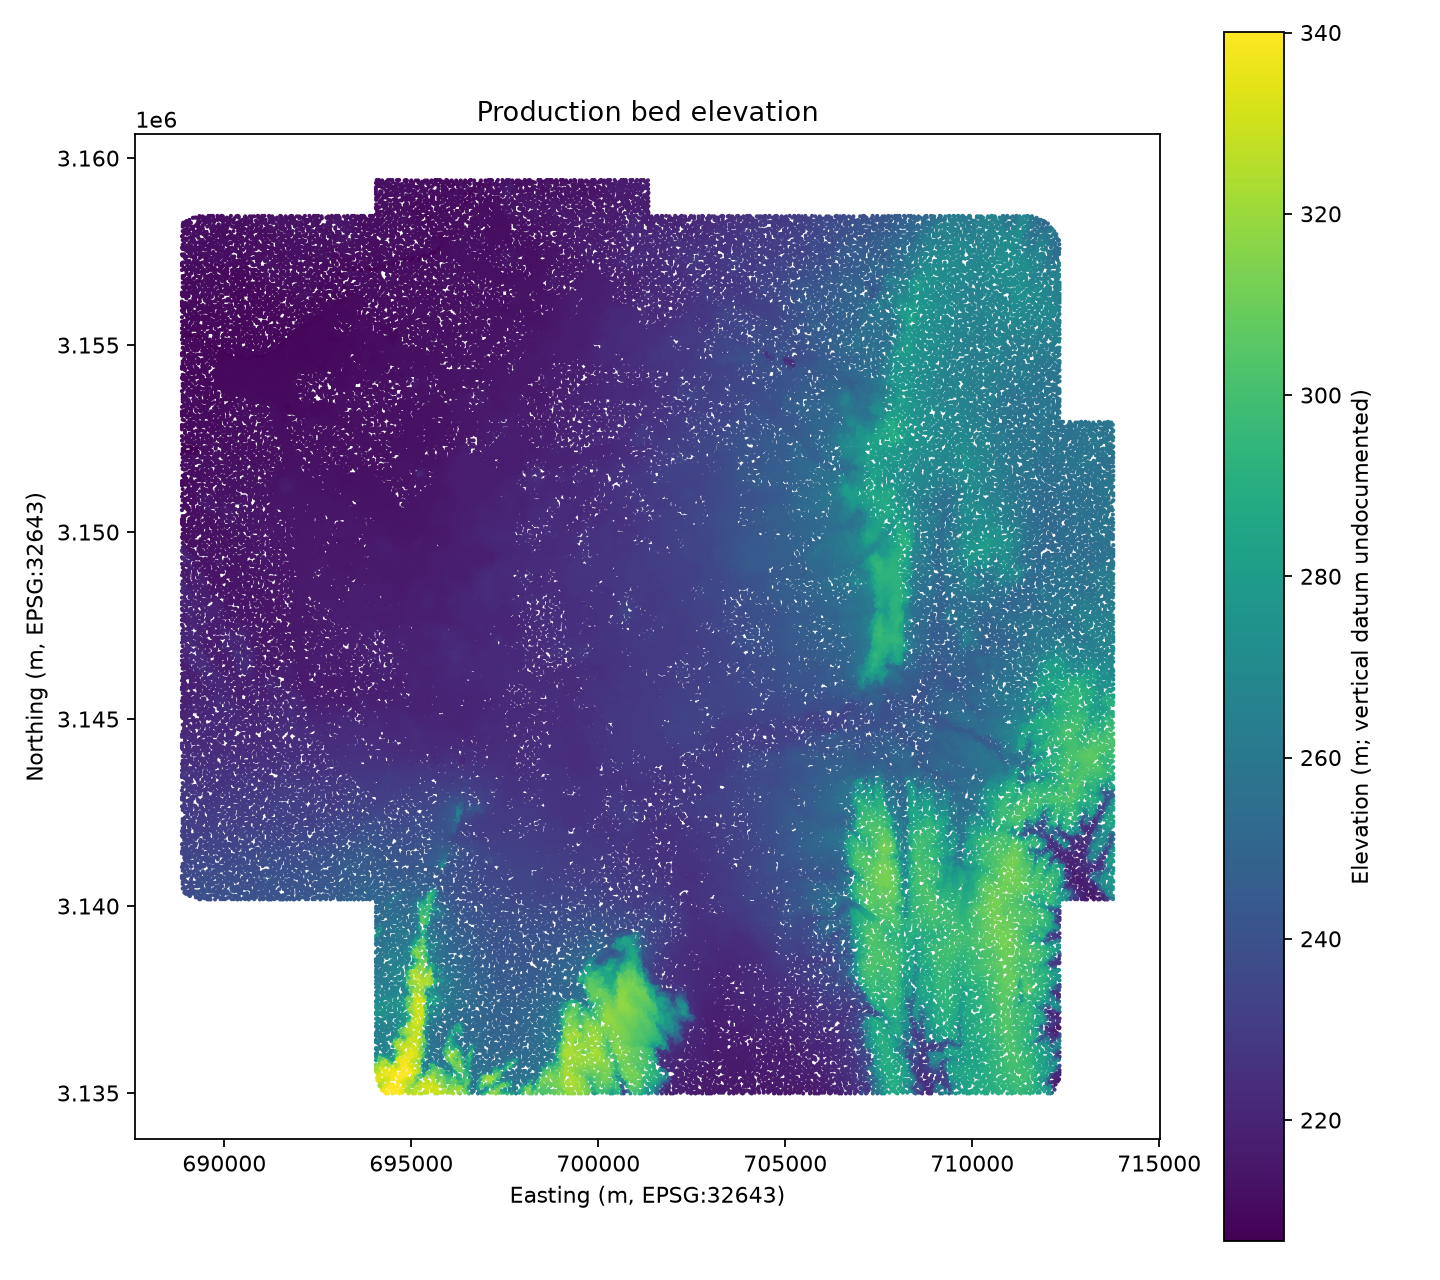
\includegraphics[width=\linewidth]{02_dem.png}
\centering{\tiny Bed elevation for all 981,880 cells}
\column{0.32\textwidth}
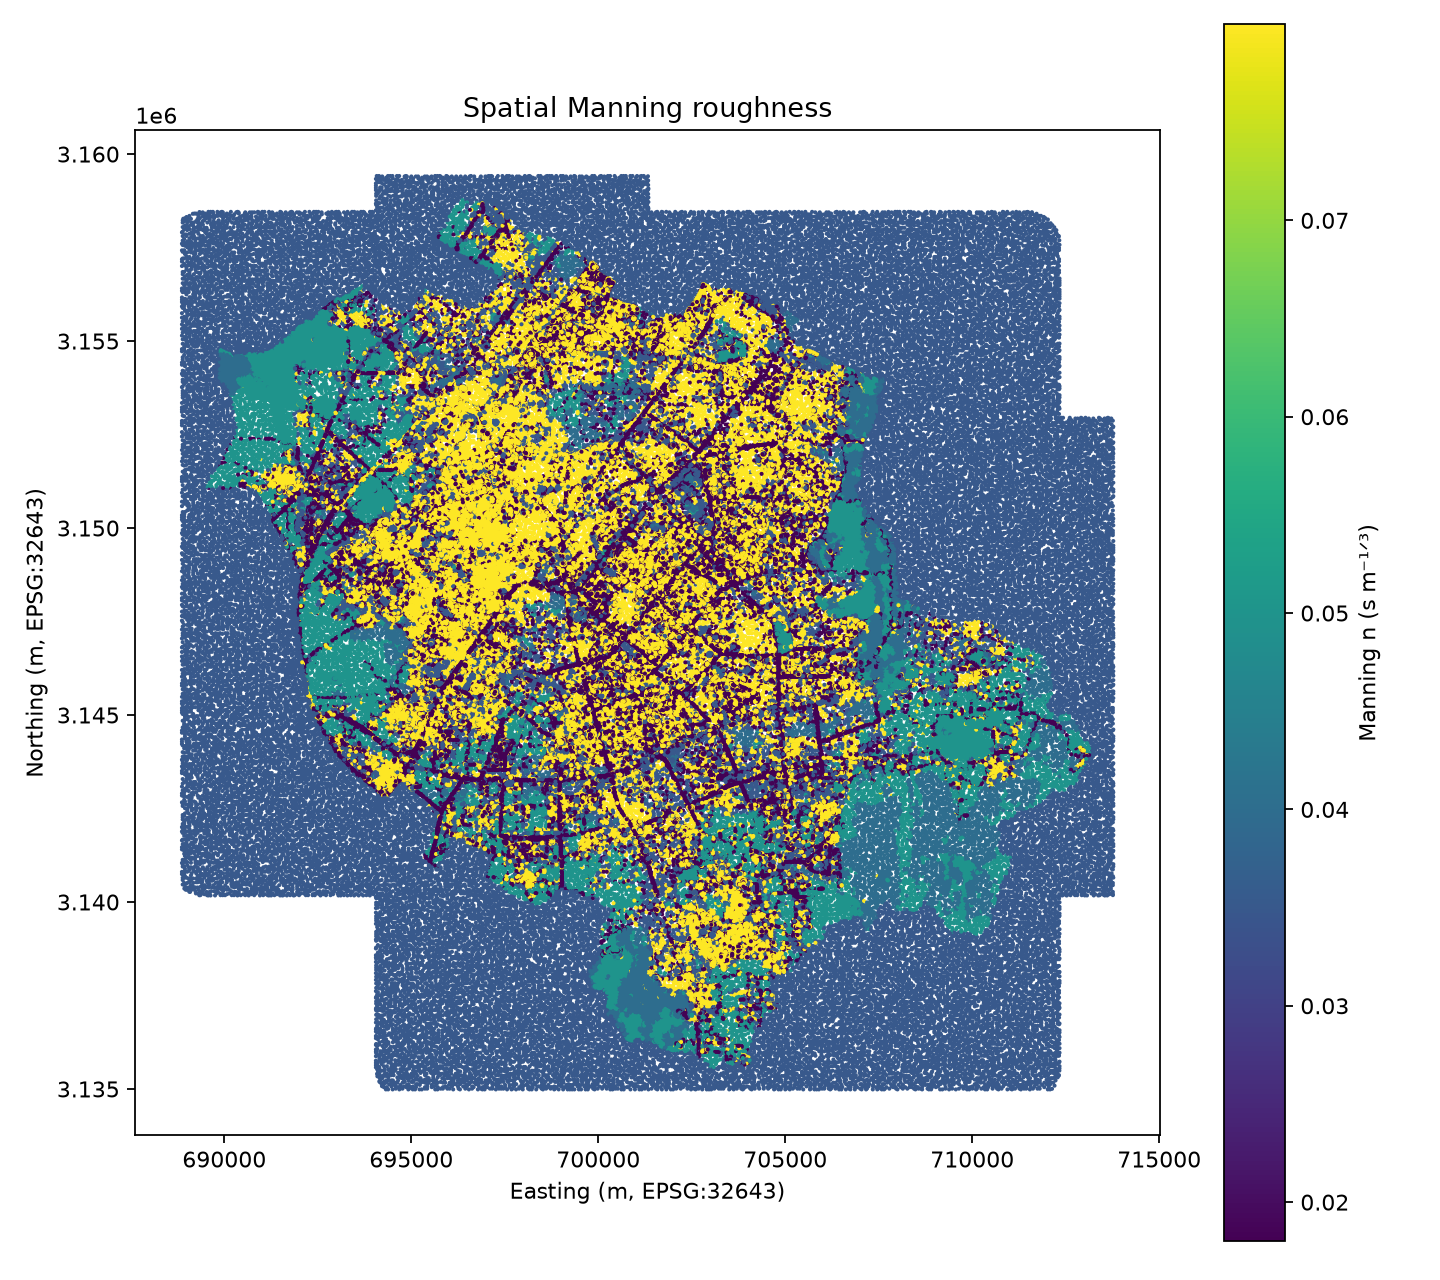
\includegraphics[width=\linewidth]{04_manning.png}
\centering{\tiny Spatial Manning $n$: 0.018--0.080}
\column{0.34\textwidth}
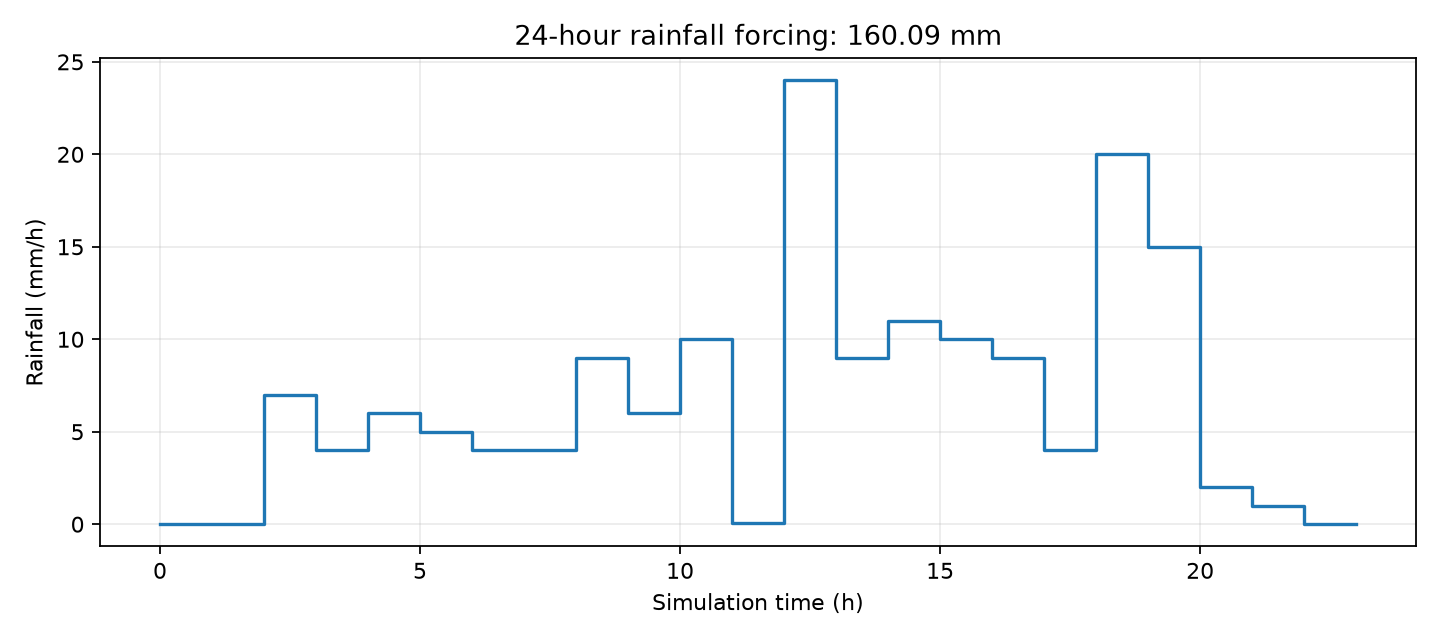
\includegraphics[width=\linewidth]{05_rainfall.png}
\centering{\tiny 24-hour rainfall: 160.09 mm}
\end{columns}

\vspace{2mm}
\small
Terrain enters hydrostatic reconstruction and hydraulic head. Manning resistance is active
friction, not metadata. Rainfall is hourly piecewise constant and spatially uniform, while
Horton losses are spatially heterogeneous: $f_0=0.0128$--7.2 mm h$^{-1}$,
$f_c=0.004$--2.25 mm h$^{-1}$ and $k=4$ h$^{-1}$.
\evsource
\end{frame}

% 5
\begin{frame}{4. Coupled surface, drainage and boundary processes}
\begin{columns}[T,onlytextwidth]
\column{0.48\textwidth}
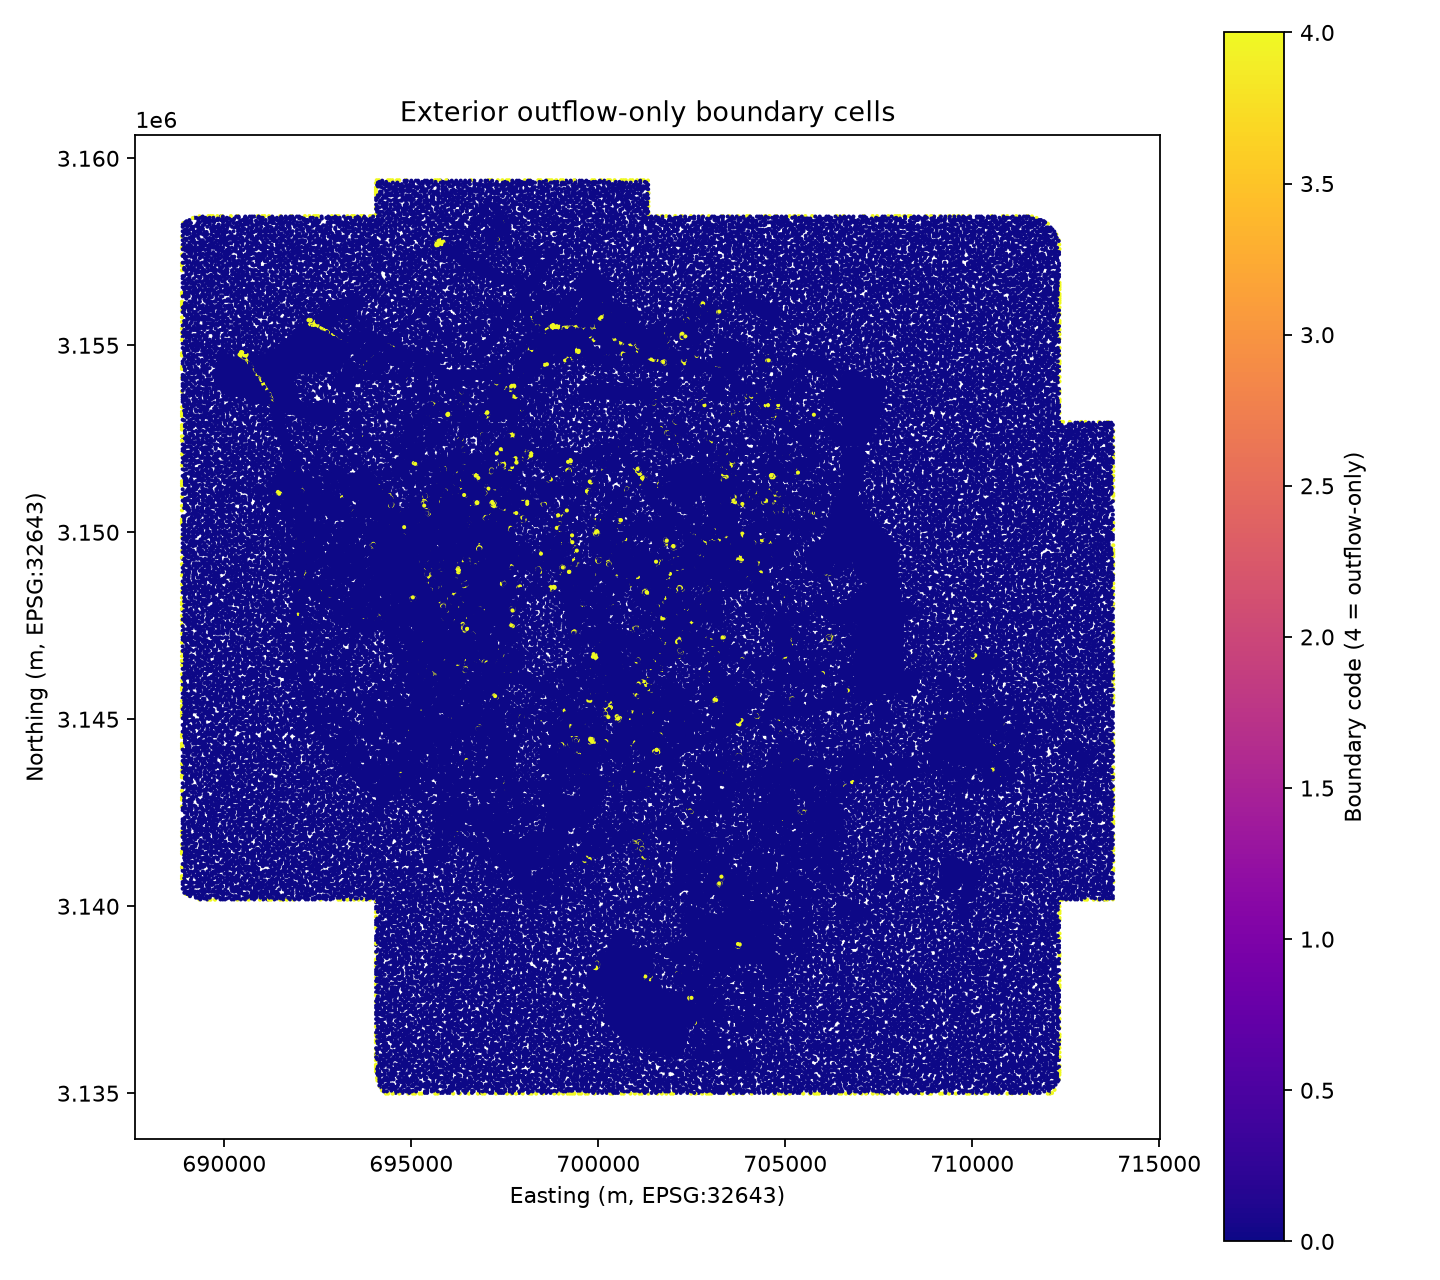
\includegraphics[width=\linewidth,height=0.62\textheight,keepaspectratio]{08_boundaries.png}
\centering{\tiny Exterior code-4 outflow-only boundary locations}
\column{0.49\textwidth}
\small
\begin{block}{Surface--node exchange}
\[
Q_e=C_dA_e\sqrt{2g\lvert H_s-H_n\rvert}\,
\operatorname{sgn}(H_s-H_n)
\]
\end{block}
Water can enter mapped inlets, move through capacity-limited links, discharge through
outfalls, or return to the surface as surcharge. Recharge captures eligible surface water
and tracks storage and removal.

\vspace{2mm}
Inactive neighbours behave as reflective walls. Exterior code-4 edges allow outward flux;
the prescribed hydrograph is applied separately to 150 receiver cells. Its recorded peak
total flow is 95.1714 m$^3$ s$^{-1}$.
\end{columns}
\evsource
\end{frame}

% 6
\begin{frame}{5. Governing physics and source terms}
\small
The conserved surface state is $\bm U=[h,hu,hv]^{\mathsf T}$ and obeys
\[
\frac{\partial\bm U}{\partial t}+\frac{\partial\bm F}{\partial x}
+\frac{\partial\bm G}{\partial y}=\bm S,
\quad
\bm F=\begin{bmatrix}hu\\hu^2+\tfrac12gh^2\\huv\end{bmatrix},\quad
\bm G=\begin{bmatrix}hv\\huv\\hv^2+\tfrac12gh^2\end{bmatrix}.
\]

\begin{columns}[T,onlytextwidth]
\column{0.49\textwidth}
\begin{block}{Horton infiltration}
\[
f(\tau)=f_c+(f_0-f_c)e^{-k\tau}
\]
Actual removal is limited by capacity and available surface water.
\end{block}
\column{0.49\textwidth}
\begin{block}{Semi-implicit Manning friction}
\[
\bm q^{n+1}=\frac{\bm q^*}{1+\Delta t\,g n^2
\lVert\bm u^*\rVert/\max(h,h_{\min})^{4/3}}
\]
Here $\bm q=(hu,hv)$ and $h_{\min}=10^{-5}$ m.
\end{block}
\end{columns}
\end{frame}

% 7
\begin{frame}{6. Finite-volume method and stable update}
\small
For triangular cell $i$ with area $A_i$,
\[
\bm U_i^{n+1}=\bm U_i^n-\frac{\Delta t}{A_i}
\sum_{e\in\partial i}L_e\widehat{\bm F}_{e,i}+\Delta t\,\bm S_i.
\]
The HLL interface flux uses left/right signal speeds $s_L,s_R$:
\[
\widehat{\bm F}_{\rm HLL}=
\frac{s_R\bm F_L-s_L\bm F_R+s_Ls_R(\bm U_R-\bm U_L)}{s_R-s_L}.
\]

\begin{columns}[T,onlytextwidth]
\column{0.49\textwidth}
\textbf{Well-balanced terrain treatment}
\small
\[
\begin{aligned}
z^*&=\max(z_L,z_R),\\
h_L^*&=\max(h_L+z_L-z^*,0),\\
h_R^*&=\max(h_R+z_R-z^*,0).
\end{aligned}
\]
\column{0.49\textwidth}
\textbf{Adaptive timestep}
\small
\[
\Delta t=\min\!\left[1\ \mathrm{s},\;0.85\min_i
\frac{\ell_i}{\lVert\bm u_i\rVert+\sqrt{gh_i}}\right].
\]
\end{columns}
\vspace{1mm}
Flux, friction, rainfall, infiltration, boundary input, network exchange, outfall, surcharge
and recharge are applied in the same order in both backends.
\end{frame}

% 8
\begin{frame}{7. Two GPU implementations of one model}
\begin{columns}[T,onlytextwidth]
\column{0.48\textwidth}
\begin{block}{CuPy/CUDA}
Device-resident NumPy-style arrays with fused custom CUDA kernels for surface and drainage
operations. Recorded implementation:
\texttt{gurugram\_flood\_backend\_fused\_cuda}.
\end{block}
\column{0.48\textwidth}
\begin{block}{JAX/XLA}
Immutable array state, scatter reductions and an XLA-compiled \texttt{while\_loop}.
Recorded implementation:
\texttt{hybrid\_flood\_v2\_jax\_v1\_parity}.
\end{block}
\end{columns}

\small
\begin{tabularx}{\textwidth}{@{}lXX@{}}
\toprule
& \textbf{CuPy} & \textbf{JAX}\\
\midrule
Execution device & CUDA device 0 & \texttt{cuda:0}\\
Production steps & 321,645 & 321,640\\
Surface precision & float32 & float32\\
GPU fallback & none & none\\
\bottomrule
\end{tabularx}

\vspace{2mm}
\textbf{Platform:} NVIDIA RTX PRO 4000 Blackwell, 24,467 MiB; driver 595.84. PyTorch CUDA
availability was recorded, but PyTorch did not execute the reported production experiment.
\evsource
\end{frame}

% 9
\begin{frame}{8. Verification and experimental protocol}
\begin{columns}[T,onlytextwidth]
\column{0.49\textwidth}
\begin{block}{24-hour production verification}
Same hashed inputs, float32 state, CFL 0.85, 1 s maximum timestep, 5 m s$^{-1}$ velocity
ceiling and 25 stored states. CuPy is the implementation reference; it is not observational
truth.
\end{block}
\textbf{Eight gates:} depth RMSE, flood CSI, volume error, finite/non-negative depth,
mass-residual regression, maximum depth, time alignment and source--sink ledger agreement.
\column{0.47\textwidth}
\begin{block}{Completed software baseline}
\centering
\Large\textbf{111 passed}\par
\normalsize 37 explicit skips; 0 failures; 0 errors
\end{block}
\begin{block}{Secondary performance protocol}
Identical 60-minute production workload; three warm-ups and ten synchronized measurements
per backend. Every timed output passed correctness checks.
\end{block}
\end{columns}
\evsource
\end{frame}

% 10
\begin{frame}{9. Production inundation results}
\begin{columns}[T,onlytextwidth]
\column{0.50\textwidth}
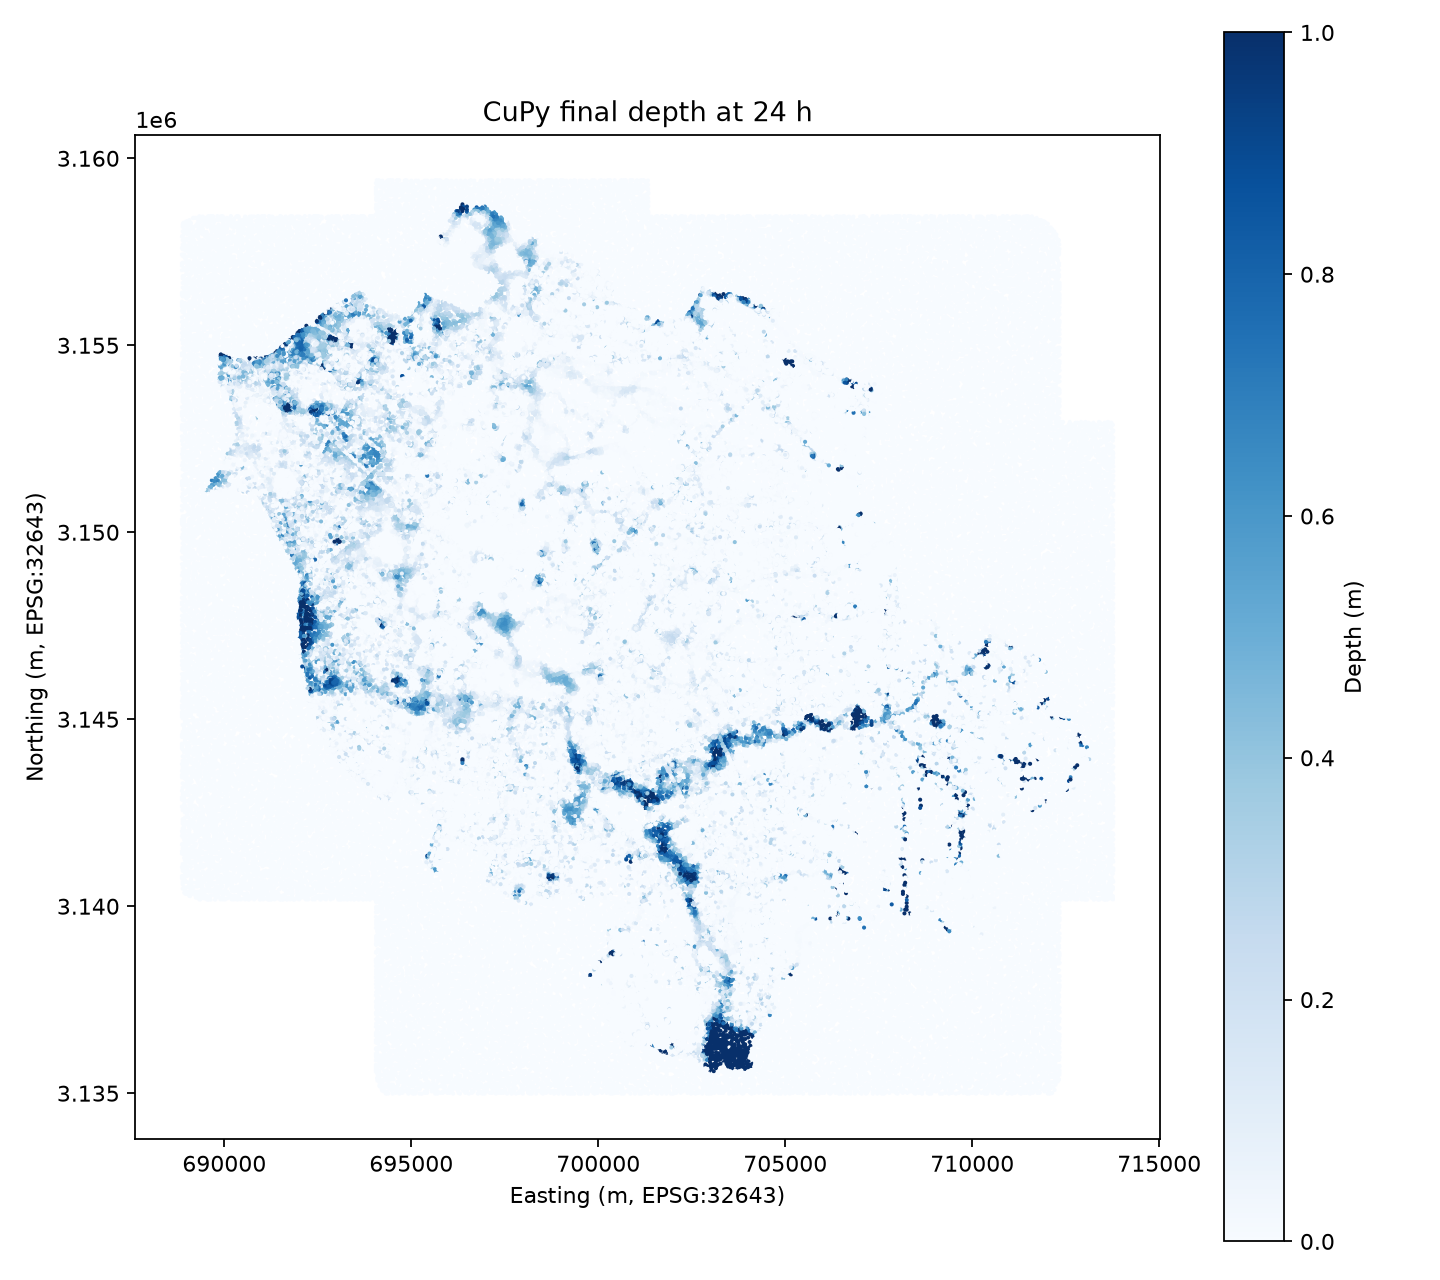
\includegraphics[width=\linewidth,height=0.62\textheight,keepaspectratio]{09_final_depth_cupy.png}
\centering{\tiny Final surface depth after 24 hours}
\column{0.50\textwidth}
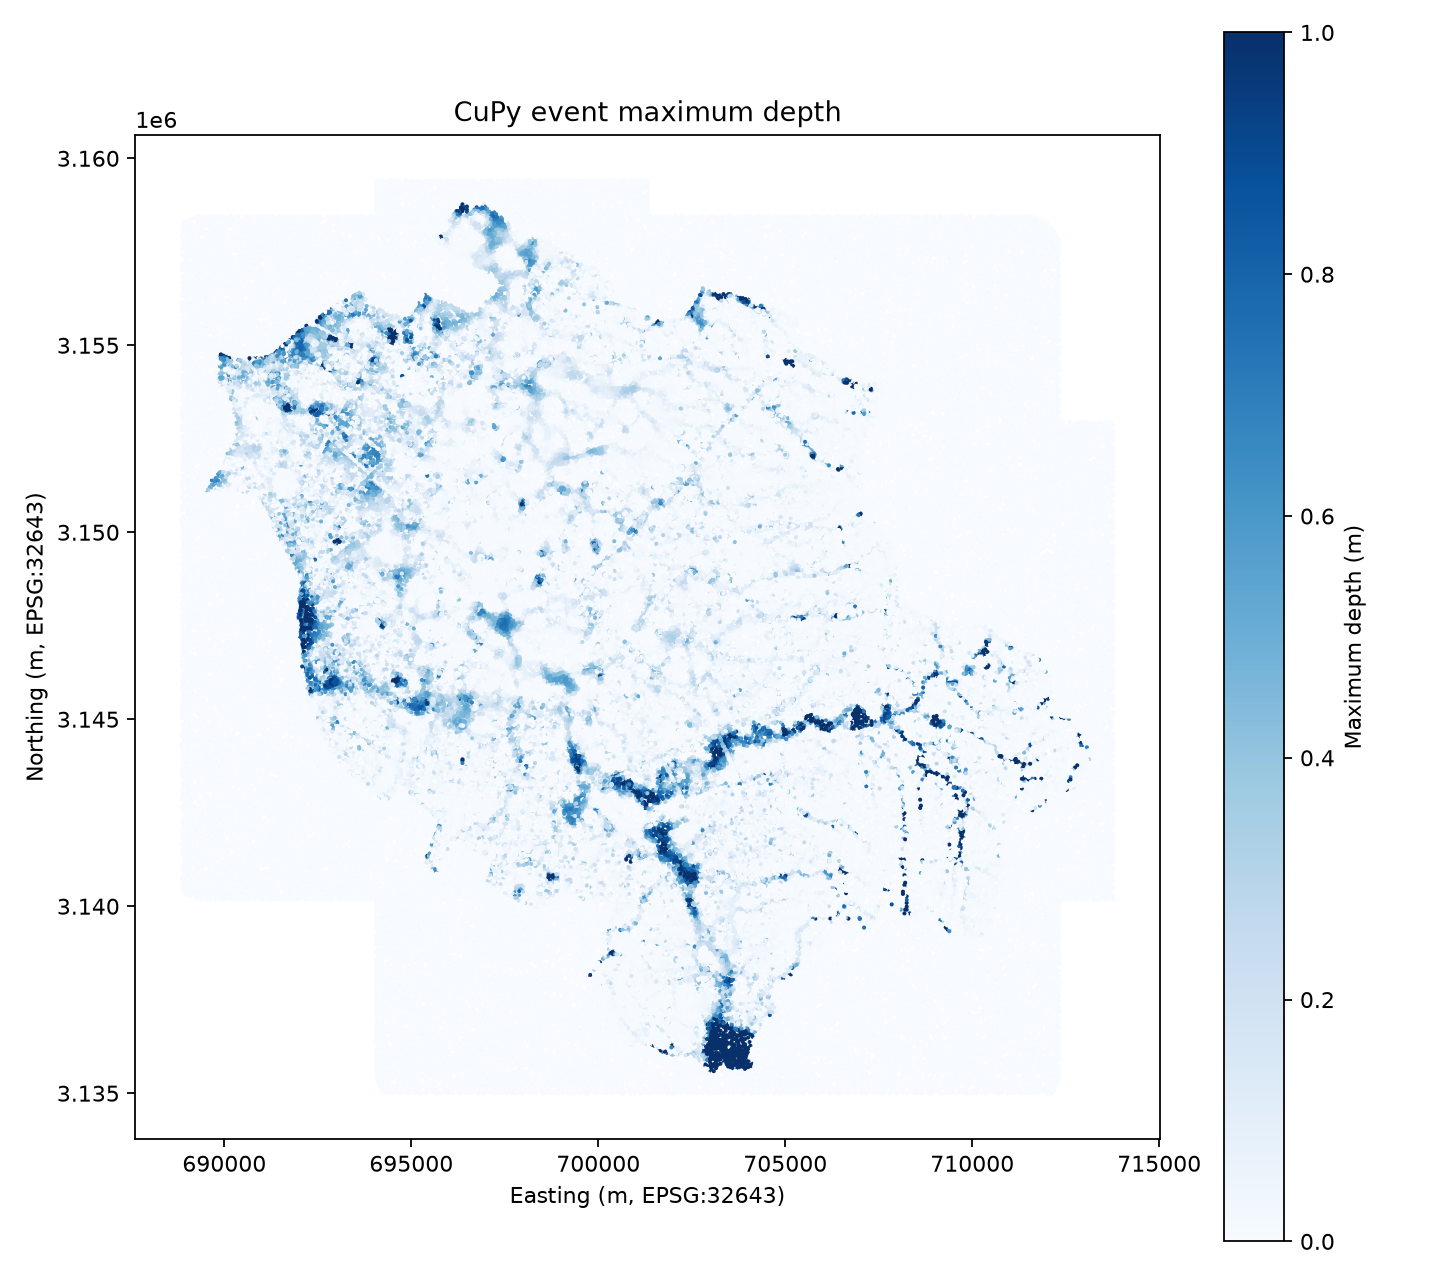
\includegraphics[width=\linewidth,height=0.62\textheight,keepaspectratio]{10_maximum_depth_cupy.png}
\centering{\tiny Event maximum surface depth}
\end{columns}
\vspace{2mm}
\centering\small
\textbf{CuPy:} maximum depth 9.414836884 m; 129,187 final wet triangles.\quad
\textbf{JAX:} maximum depth 9.414829254 m; 129,180 final wet triangles.
\evsource
\end{frame}

% 11
\begin{frame}{10. Flood extent, arrival and duration}
\begin{columns}[T,onlytextwidth]
\column{0.333\textwidth}
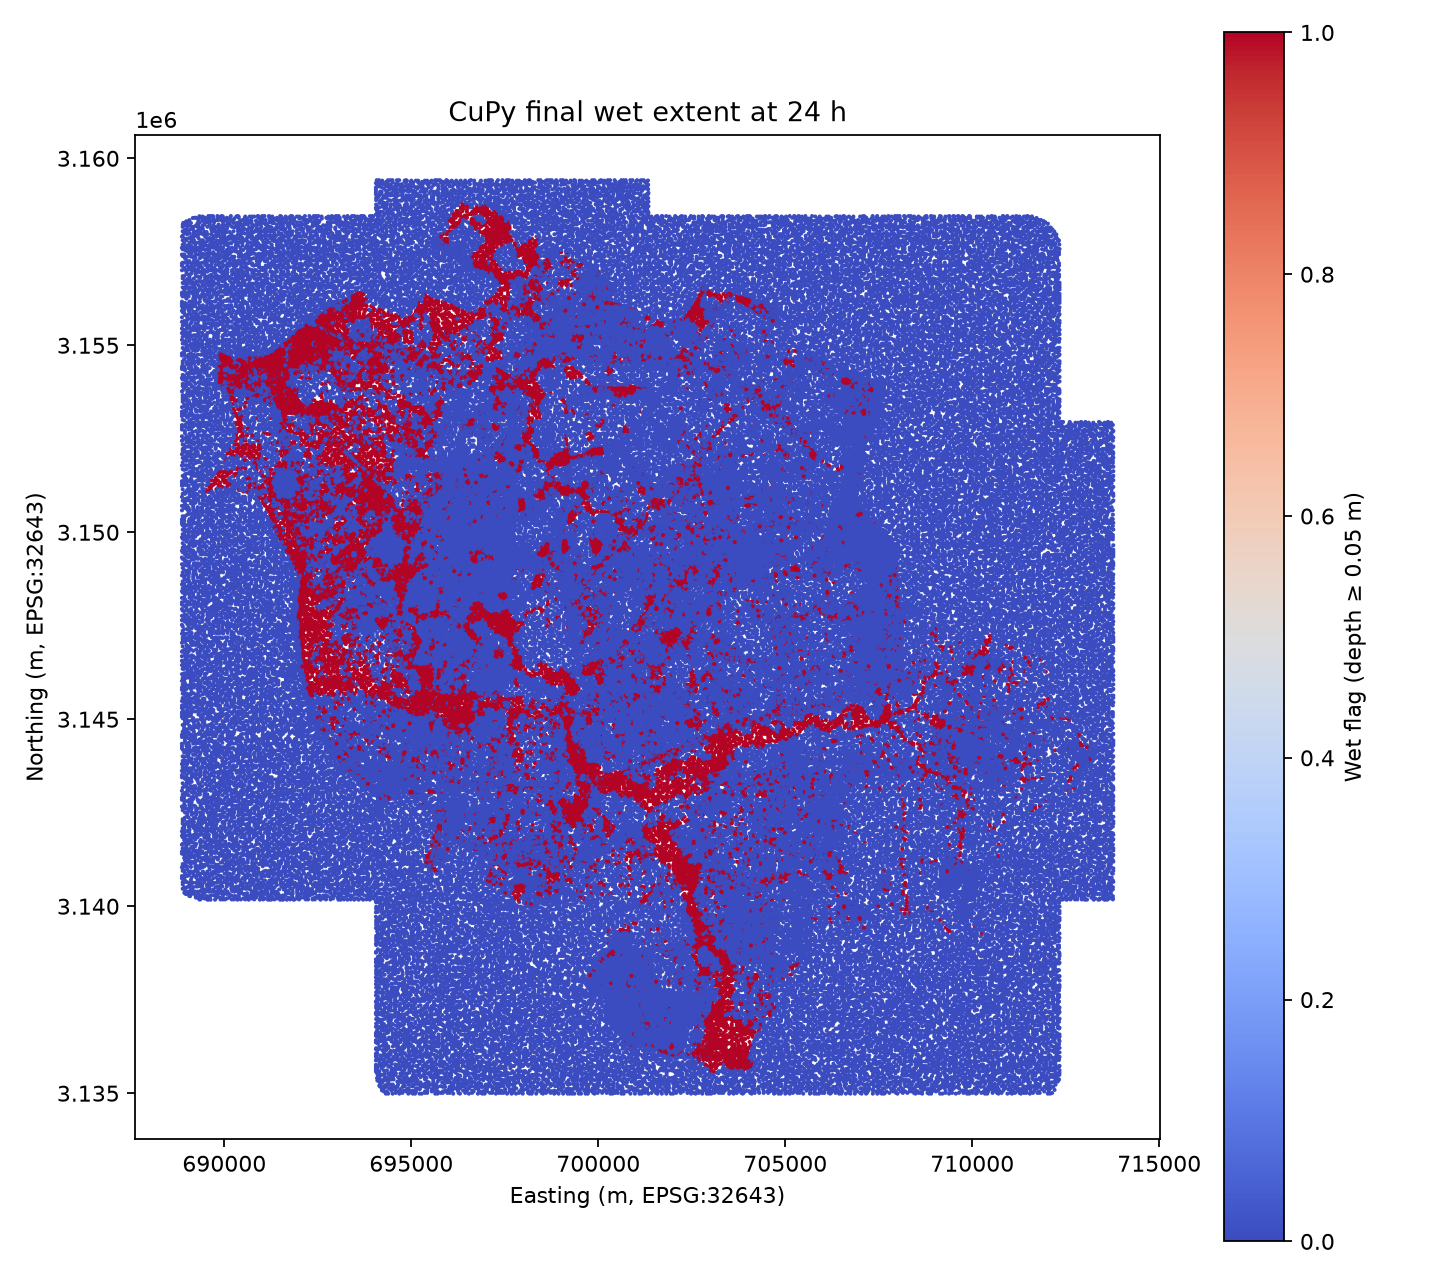
\includegraphics[width=\linewidth]{11_wet_extent.png}
\centering{\tiny Wet extent through the event}
\column{0.333\textwidth}
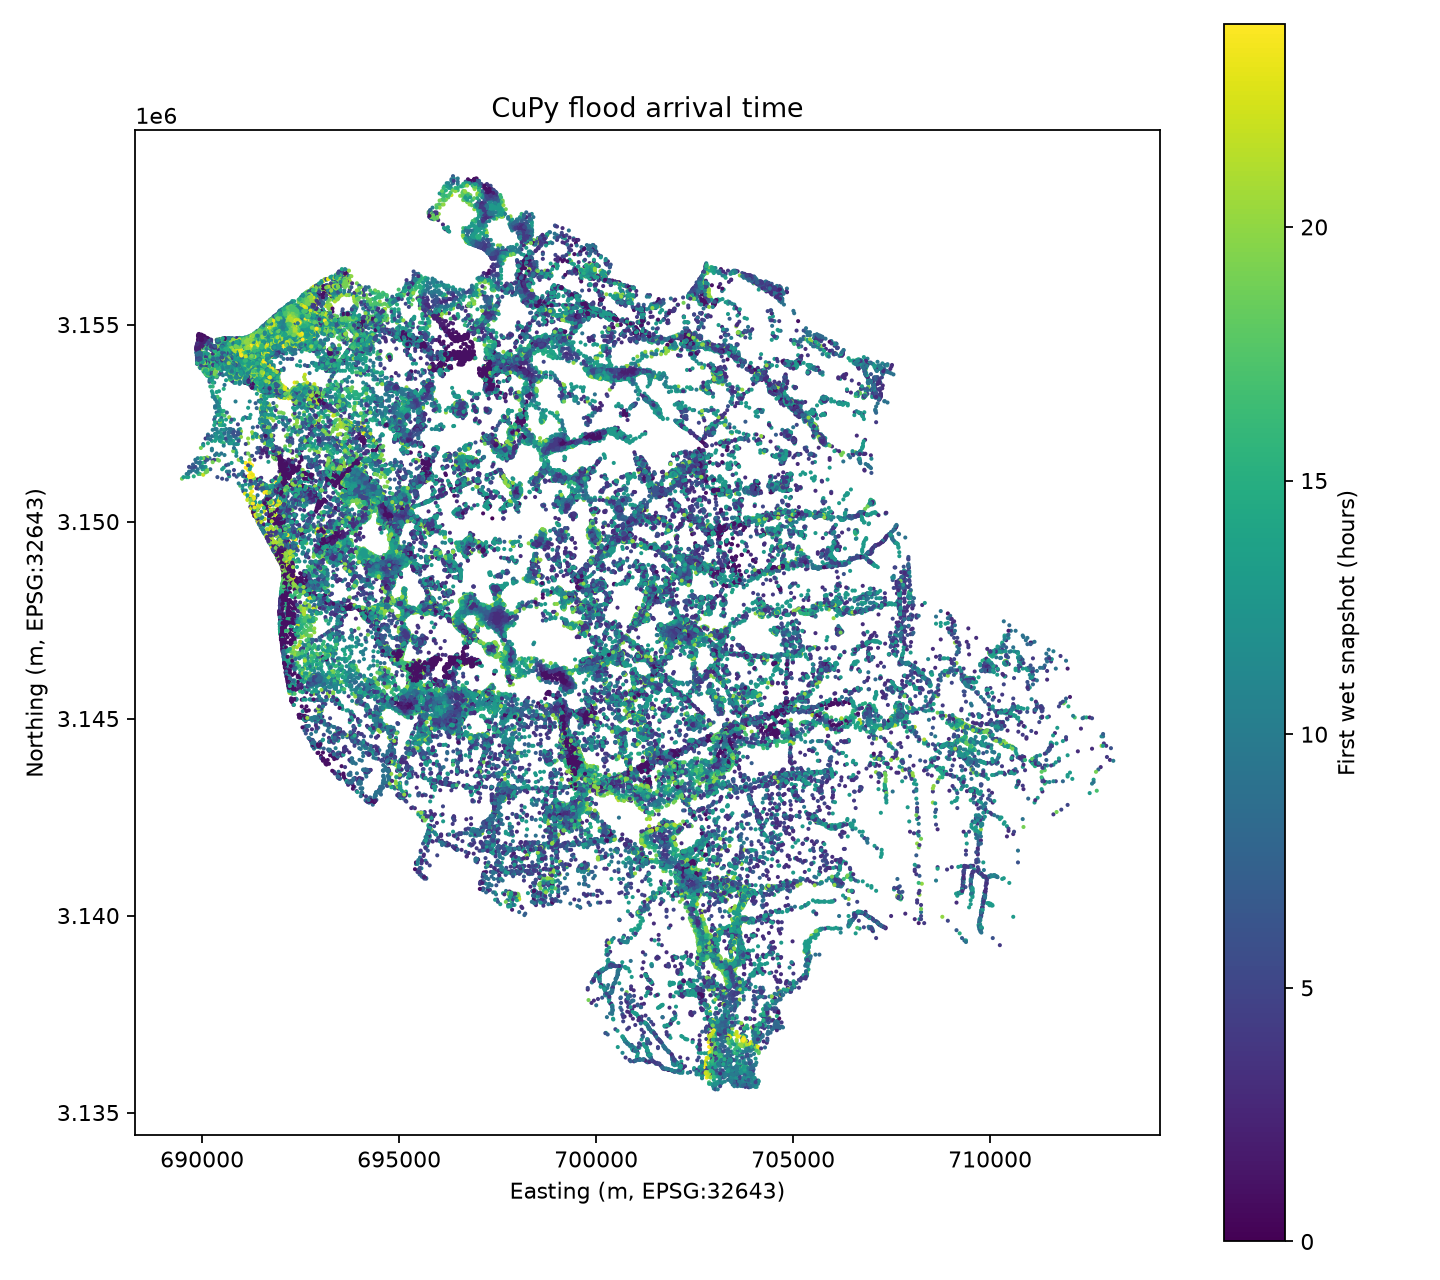
\includegraphics[width=\linewidth]{12_arrival_time.png}
\centering{\tiny Arrival time at $h>0.05$ m}
\column{0.333\textwidth}
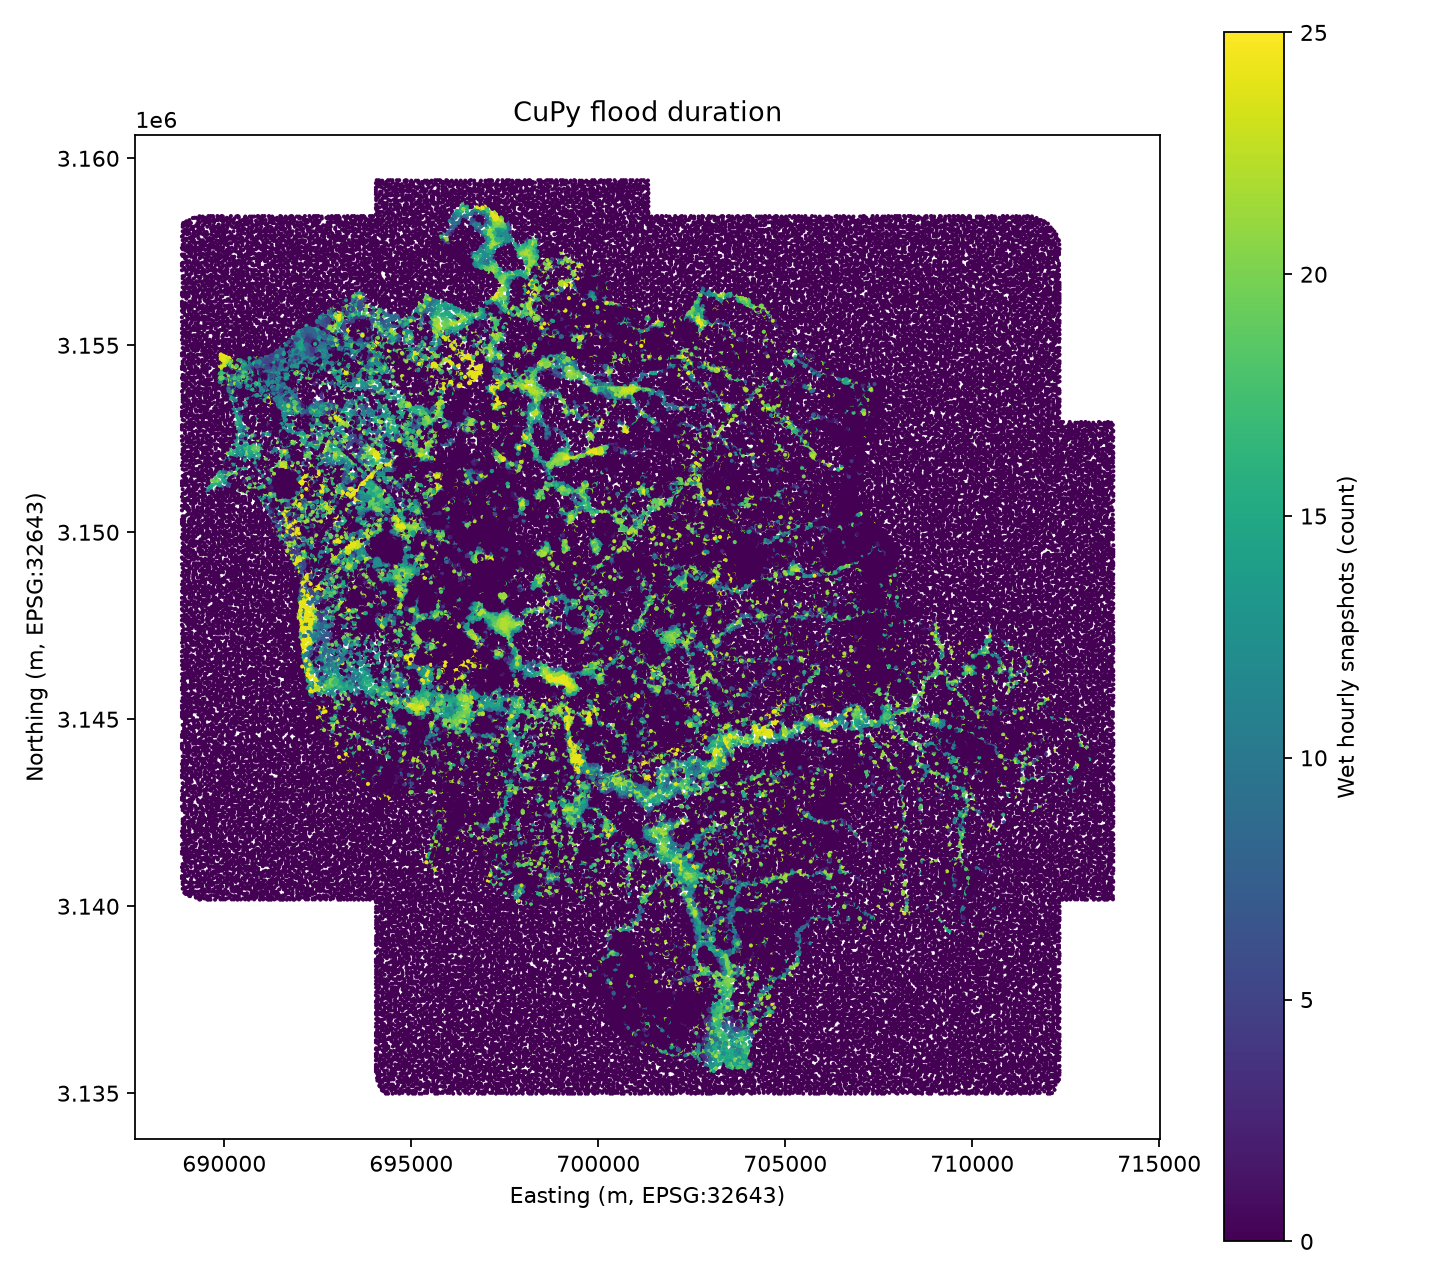
\includegraphics[width=\linewidth]{13_flood_duration.png}
\centering{\tiny Number of wet stored states}
\end{columns}

\vspace{2mm}
\small
Flood extent uses the registered 0.05 m threshold. Arrival and duration are derived from 25
stored states, so their effective temporal resolution is hourly. The duration product is a
wet-snapshot count, not a continuously integrated exposure duration.
\evsource
\end{frame}

% 12
\begin{frame}{11. Velocity, storage and coupled mass response}
\begin{columns}[T,onlytextwidth]
\column{0.39\textwidth}
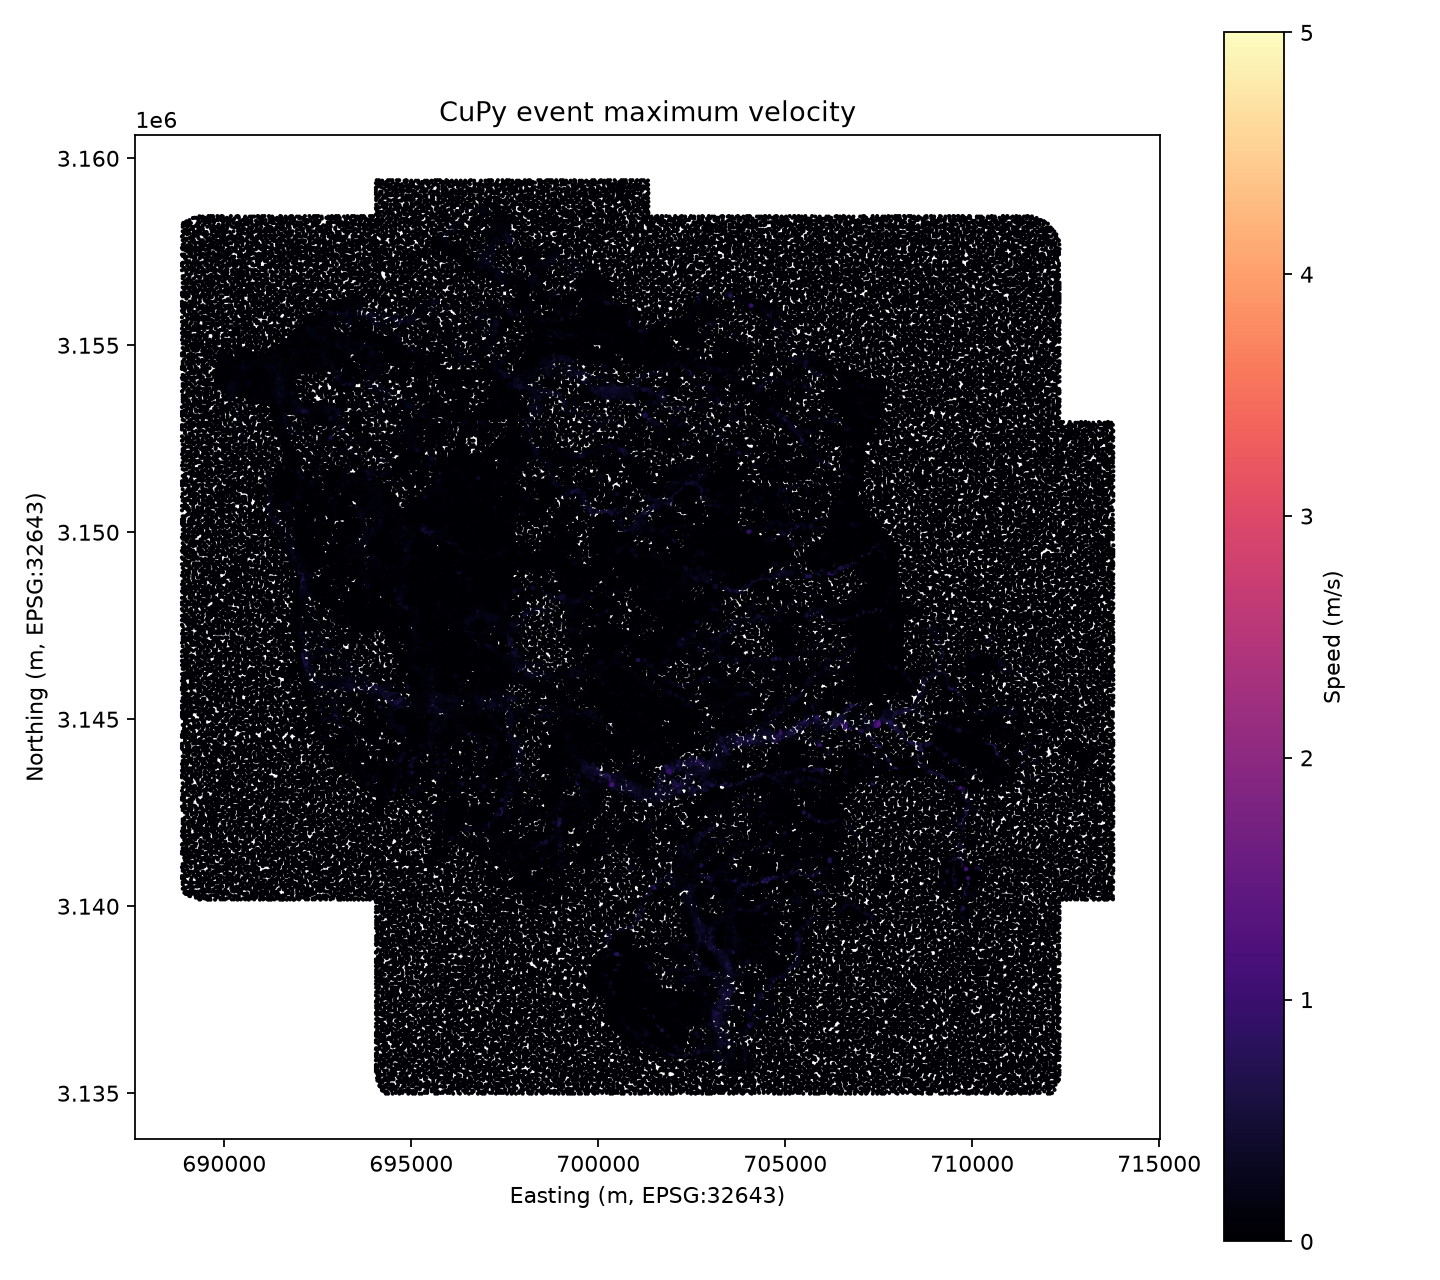
\includegraphics[width=\linewidth,height=.37\textheight,keepaspectratio]{14_velocity.png}
\centering{\tiny CuPy event maximum velocity}
\column{0.59\textwidth}
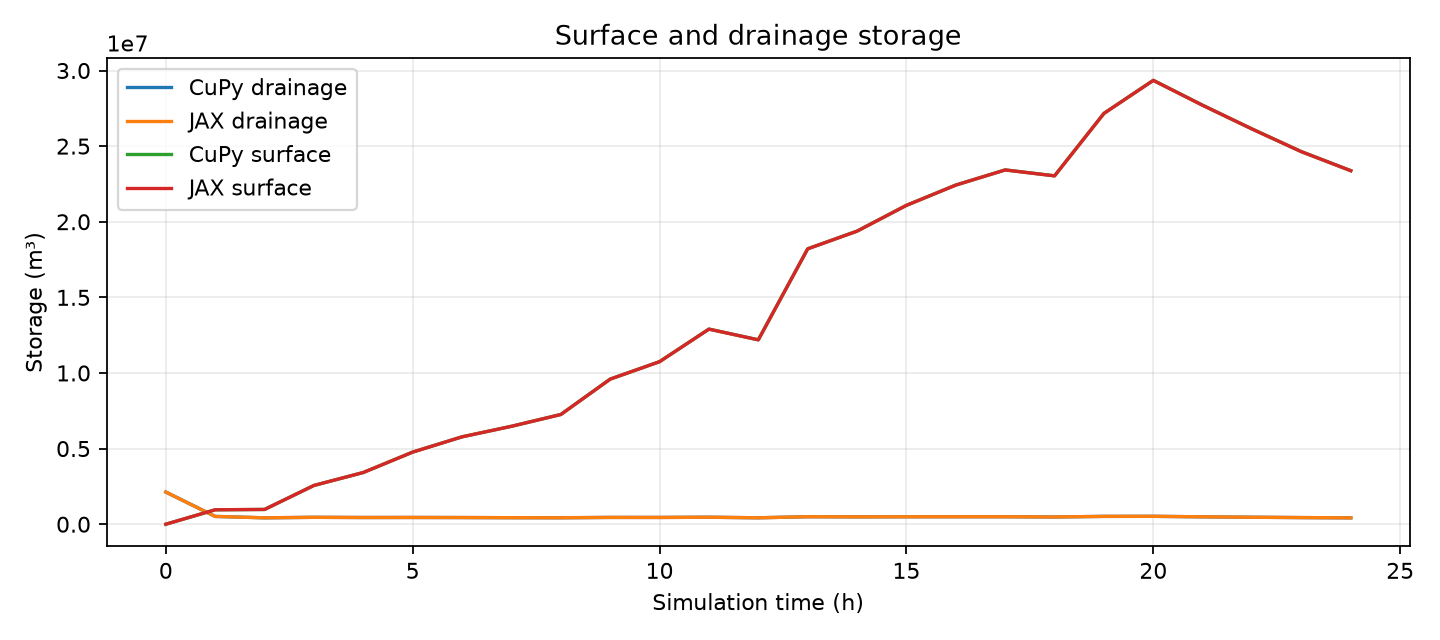
\includegraphics[width=\linewidth,height=.37\textheight,keepaspectratio]{15_storage.png}
\centering{\tiny Surface and drainage-node storage}
\end{columns}

\vspace{1mm}
\small
Maximum recorded speed was 1.712713 m s$^{-1}$ for CuPy and 1.712712 m s$^{-1}$ for JAX,
below the 5 m s$^{-1}$ safety ceiling. Final surface storage was 23.378 and
23.376 million m$^3$; final drainage-node storage was 0.4204 million m$^3$ in both paths.

\[
R_M=V_{s,0}+V_{n,0}+\sum V_{\rm in}-\sum V_{\rm loss}-V_{s,f}-V_{n,f}-V_{r,f}.
\]
\evsource
\end{frame}

% 13
\begin{frame}{12. Cross-backend numerical parity}
\begin{columns}[T,onlytextwidth]
\column{0.33\textwidth}
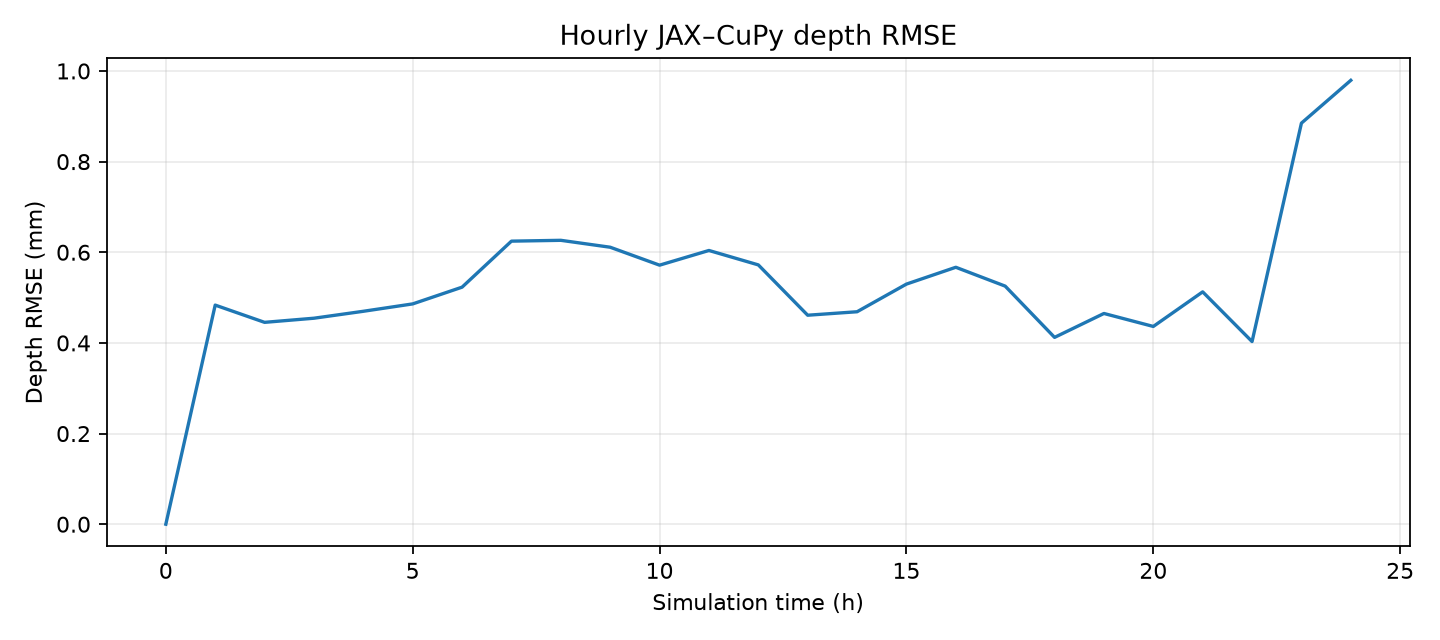
\includegraphics[width=\linewidth,height=.31\textheight,keepaspectratio]{16_parity_rmse.png}
\centering{\tiny Hourly depth RMSE}
\column{0.33\textwidth}
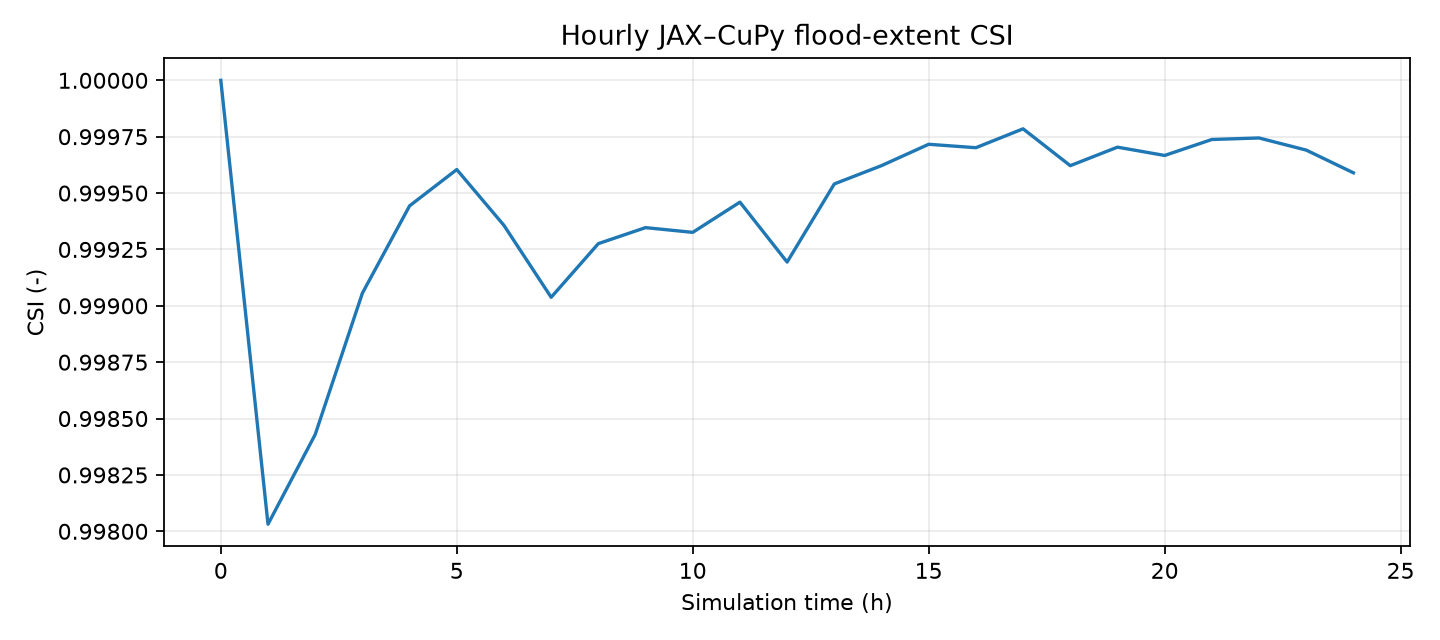
\includegraphics[width=\linewidth,height=.31\textheight,keepaspectratio]{17_parity_csi.png}
\centering{\tiny Hourly flood-extent CSI}
\column{0.33\textwidth}
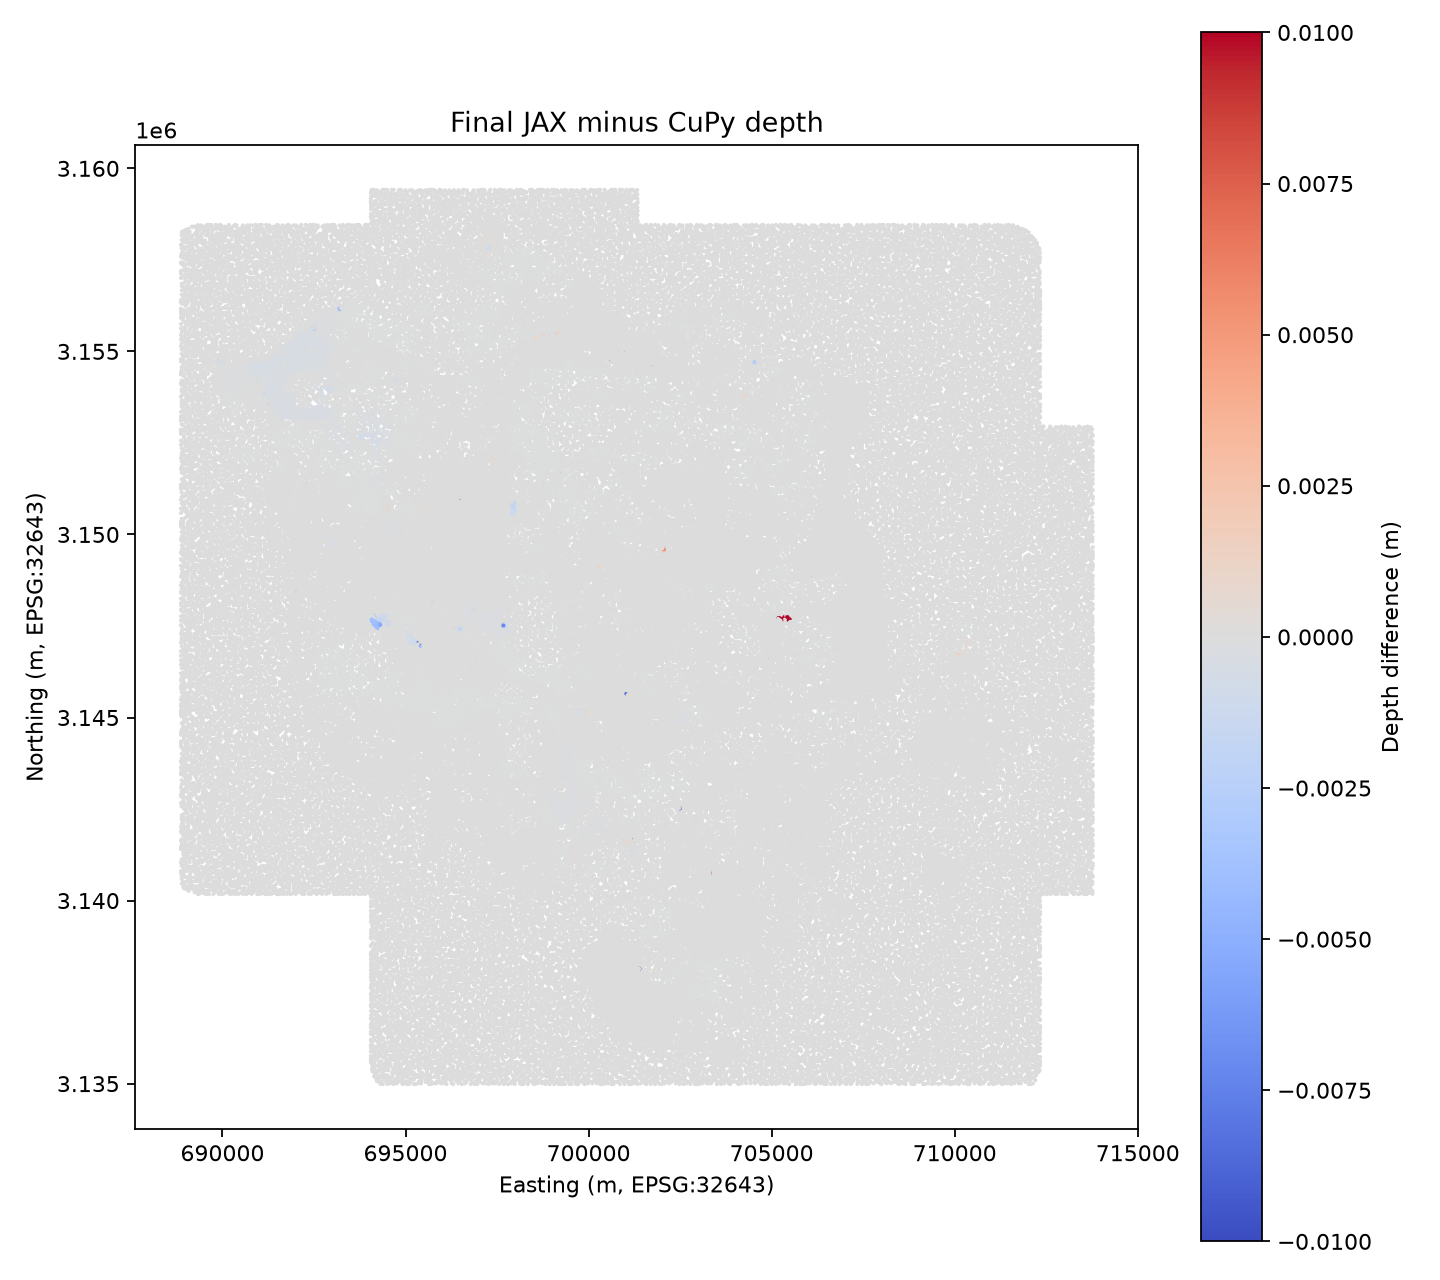
\includegraphics[width=\linewidth,height=.31\textheight,keepaspectratio]{18_spatial_depth_difference.png}
\centering{\tiny Final JAX--CuPy depth difference}
\end{columns}

\vspace{1mm}
\scriptsize
\begin{tabularx}{\textwidth}{@{}Xrrc@{}}
\toprule
\textbf{Gate} & \textbf{Limit} & \textbf{Observed} & \textbf{Result}\\
\midrule
Maximum hourly depth RMSE & $\leq0.05$ m & 0.000979348 m & Pass\\
Minimum hourly flood CSI & $\geq0.95$ & 0.998031 & Pass\\
Maximum hourly volume error & $\leq2\%$ & 0.033294\% & Pass\\
Snapshot-time mismatch & $\leq1$ s & 0.318359 s & Pass\\
Source--sink ledger difference & $\leq2\%$ & 1.543653\% & Pass\\
\bottomrule
\end{tabularx}
\centering\normalsize\color{hfgreen}\textbf{All eight registered parity gates passed.}
\evsource
\end{frame}

% 14
\begin{frame}{13. Repeatability and measured GPU performance}
\begin{columns}[T,onlytextwidth]
\column{0.44\textwidth}
\textbf{Independent 24-hour repeat runs}
\vspace{1mm}

\scriptsize
\begin{tabular}{@{}lrr@{}}
\toprule
& \textbf{CuPy} & \textbf{JAX}\\
\midrule
Depth RMSE (m) & 0.000416766 & 0.000406100\\
Minimum CSI & 0.998740 & 0.998031\\
Maximum time offset (s) & 0.354492 & 0.337891\\
Step-count difference & 28 & 24\\
Bitwise identical & No & No\\
\bottomrule
\end{tabular}

\vspace{3mm}
\small Both backends are \textbf{numerically repeatable within the approved criteria}, but
neither is bitwise deterministic.
\column{0.54\textwidth}
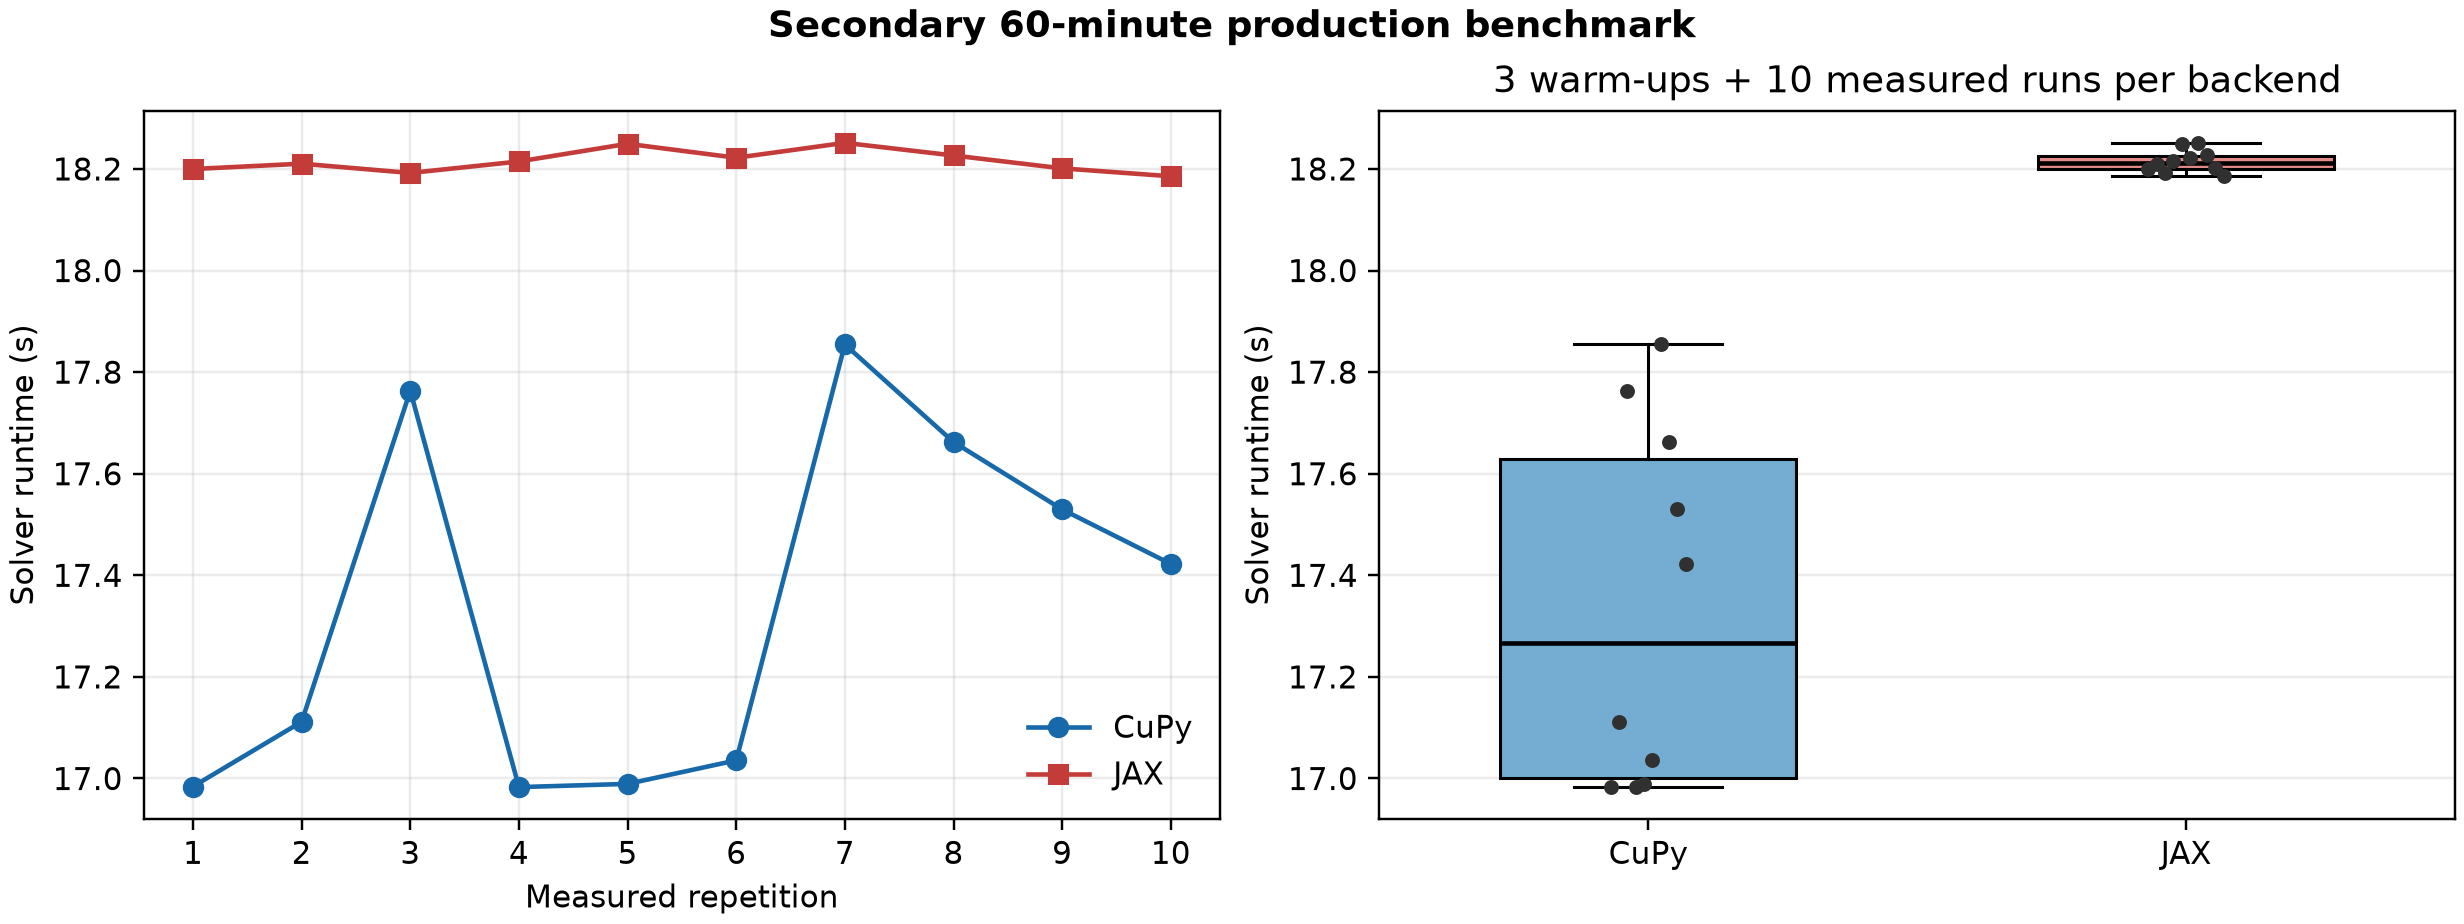
\includegraphics[width=\linewidth]{19_runtime_distribution.png}
\centering{\tiny Three warm-ups and ten measurements per backend}

\small
CuPy median: \textbf{17.267 s}\qquad JAX median: \textbf{18.213 s}

JAX was \textbf{5.476\% slower} for this specific completed 60-minute workload. All timing
correctness checks passed.
\end{columns}
\evsource
\end{frame}

% 15
\begin{frame}{14. Conclusions and defensible project claims}
\begin{block}{Primary conclusion}
\small
Equivalent CuPy/CUDA and JAX/XLA implementations successfully executed the complete
production urban flood model on one NVIDIA GPU, and all registered cross-backend numerical
gates passed.
\end{block}

\begin{columns}[T,onlytextwidth]
\column{0.48\textwidth}
\textbf{What was demonstrated}
\begin{itemize}\tightitem
\item City-scale coupled surface--drainage execution
\item Numerical parity throughout 24 hours
\item Within-backend numerical repeatability
\item Valid repeated secondary performance comparison
\end{itemize}
\column{0.48\textwidth}
\textbf{Correct scientific boundary}

The results demonstrate GPU implementation consistency, not agreement with observed flood
measurements. ANUGA is external reference context only and contributes no production result.
The incomplete repeated 24-hour timing series is not used as an official benchmark ratio.
\end{columns}

\vspace{1mm}
\centering
\color{hfblue}\large\textbf{Completed outcome: a verified, reproducible GPU numerical study.}
\evsource
\end{frame}

\end{document}
